By DC characterizing the fabricated antennas we aim to ensure ohmic behavior. The IV-characteristics of the antennas are measured by sweeping through the supply voltage from \num{-1000} \si{\milli \volt} to \num{1000} \si{\milli \volt} with a step size of \num{50} \si{\milli \volt}. Figure \ref{fig:main_IV_dipoles} shows the measured dark current $I_{DC}$ over the applied voltage $V$. Each plot displays two antennas with similar properties, meaning identical fabrication. All antennas display ohmic behavior as their IV-characteristics are strictly linear, thus $I_{DC} \sim V$ and $R = \frac{\Delta V}{\Delta I_{DC}}$. We conclude that concerning the metal-semiconductor contact, the antennas behave as expected.  

The measured resistance is generally higher than assumed in simulations. The sheet resistance can be calculated from the measurements as follows

\begin{equation}
    R_{sq} = R_{NiCr}\cdot\frac{w_{strip}}{l_{NiCr}},
\end{equation}

where $w_{strip}$ is the width of the feeding strip, $l_{NiCr}$ is the length of the NiCr portion of the strip and $R_{NiCr}$ is the measured resistance. By calculating the sheet resistance for every measurement of H-Dipole antennas with NiCr induced feeds and taking the mean, we arrive at a sheet resistance of approx. $R_{sq} = 215$ \si{\ohm/sq}. Compared to the assumptions in our simulations, the sheet resistance is approx. ten times higher than expected. The assumed sheet resistance in simulations stemmed from previous flash evaporation processes and measurements. The flash evaporation for this thesis was done at slightly lower temperatures. This results in different conductivity properties of the \num{80}/\num{20} NiCr alloy and could be a reason for the higher sheet resistance.

\textbf{TODO: REWORK !!!!}


In simulations we saw that above a few hundred ohms we should expect the low frequency resonances to reduce and ultimately disappear. With the now fabricated antennas, we expect to only observe low frequency resonances in the reference H-Dipole that does not contain NiCr. Even the antenna with the shortest NiCr-strip $L_{NiCr} = 70$ \si{\micro \meter} should already completely suppress the undesired low frequency effects caused by the pads. What happens with the resistances around \num{20} \si{\kilo \ohm} has to be evaluated in measurements. The NiCr strips act as an additional parallel resistance to the resistance of the photoconductor $R_P$ (see figure \ref{PCA_eq}). Usually, $R_P$ is in the mega ohm region and can be ignored as it is parallel to the radiation impedance $Z_A$ of the antenna. In eq. \ref{transferfunction} we assumed $R_P \gg R_A$, so $R_P$ could be neglected. With small values for $R_{NiCr}$ however, the parallel circuit of $R_P$ and $R_{NiCr}$ is

\begin{equation}
    R_{res} = R_P || R_{NiCr} = \frac{R_P\cdot R_{NiCr}}{R_P + R_{NiCr}} \approx R_{NiCr}.
\end{equation}

We cannot assume to neglect the resistance parallel to $R_A$ anymore. Inserting this result into eq. \ref{transferfunction} we get 

\begin{equation}
    H = \frac{Z_{out}}{Z_{in}} = \frac{\frac{1}{i\omega C_P}}{R_A || R_{NiCr} + \frac{1}{i\omega C_P}} = \frac{1}{1 + i\omega C_P \frac{R_A \cdot R_{NiCr}}{R_A + R_{NiCr}}} = \frac{1}{1 + i 2\pi \nu_{THz} \tau_{RC}}.   
\end{equation}

We see that the transfer function of the PCA is only influenced when $R_{NiCr}$ is sufficiently small. 

\begin{figure}[ht]
    \centering
    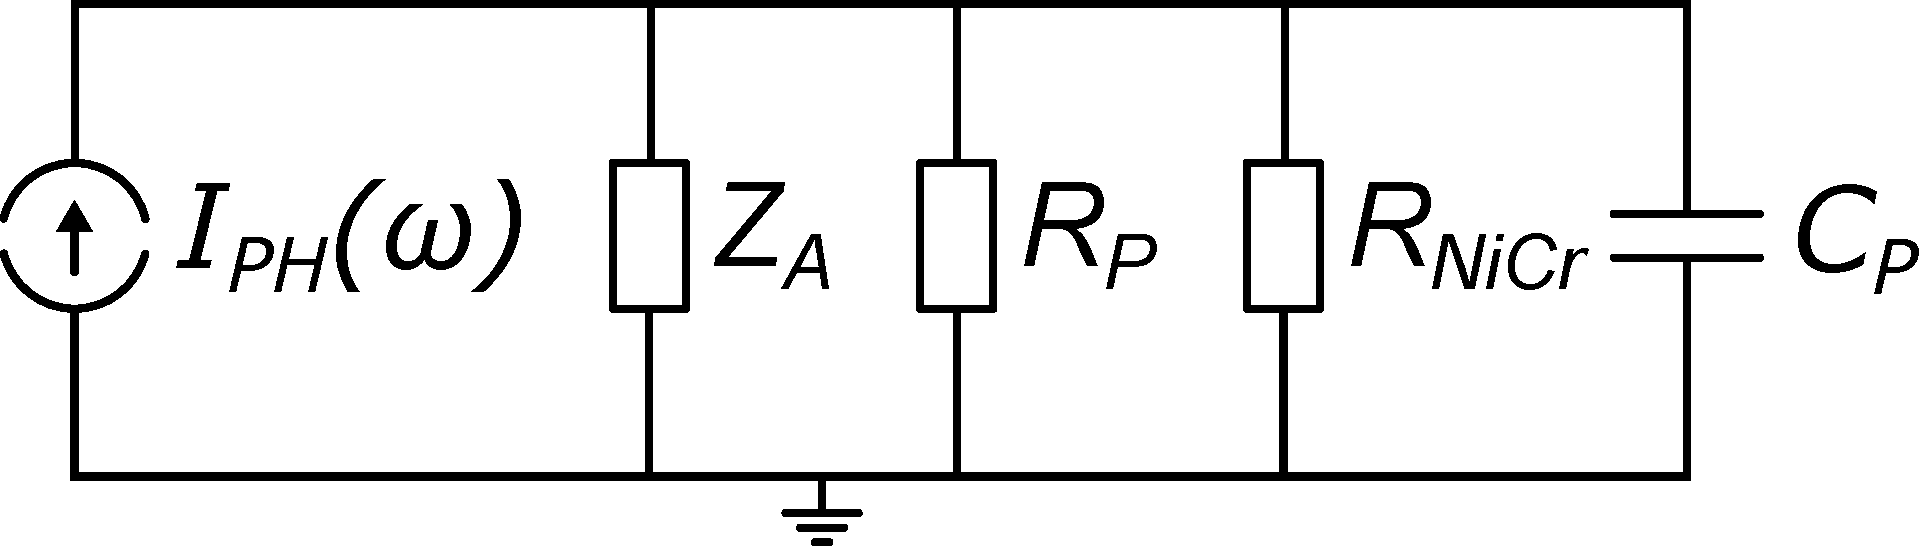
\includegraphics[width=0.7\textwidth]{figures/eq_circuit_PCA_wNiCr.pdf}
    \caption{}
    \label{eq_circuit_NiCR}
\end{figure}

\begin{figure}[ht]
    \centering

    \begin{subfigure}[b]{0.49\textwidth}
        \centering
        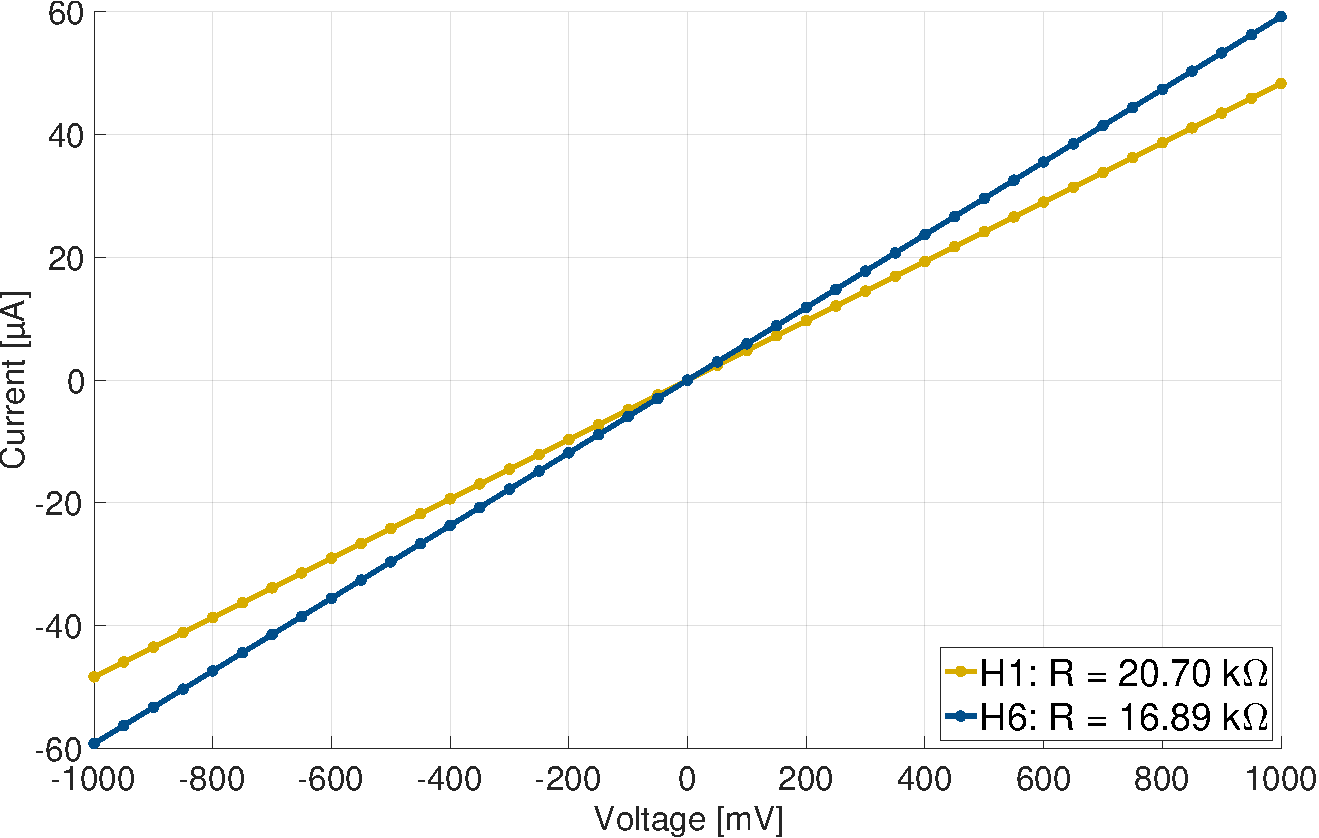
\includegraphics[width=\textwidth]{figures/IV/IV_H1_H6.pdf}
        \caption{IV characteristics of H-Dipole antennas with a NiCr-strip of length $l_{NiCr} = 500$ \si{\micro \meter}.}
        \label{fig:sub1}
    \end{subfigure}
    \hfill
    \begin{subfigure}[b]{0.49\textwidth}
        \centering
        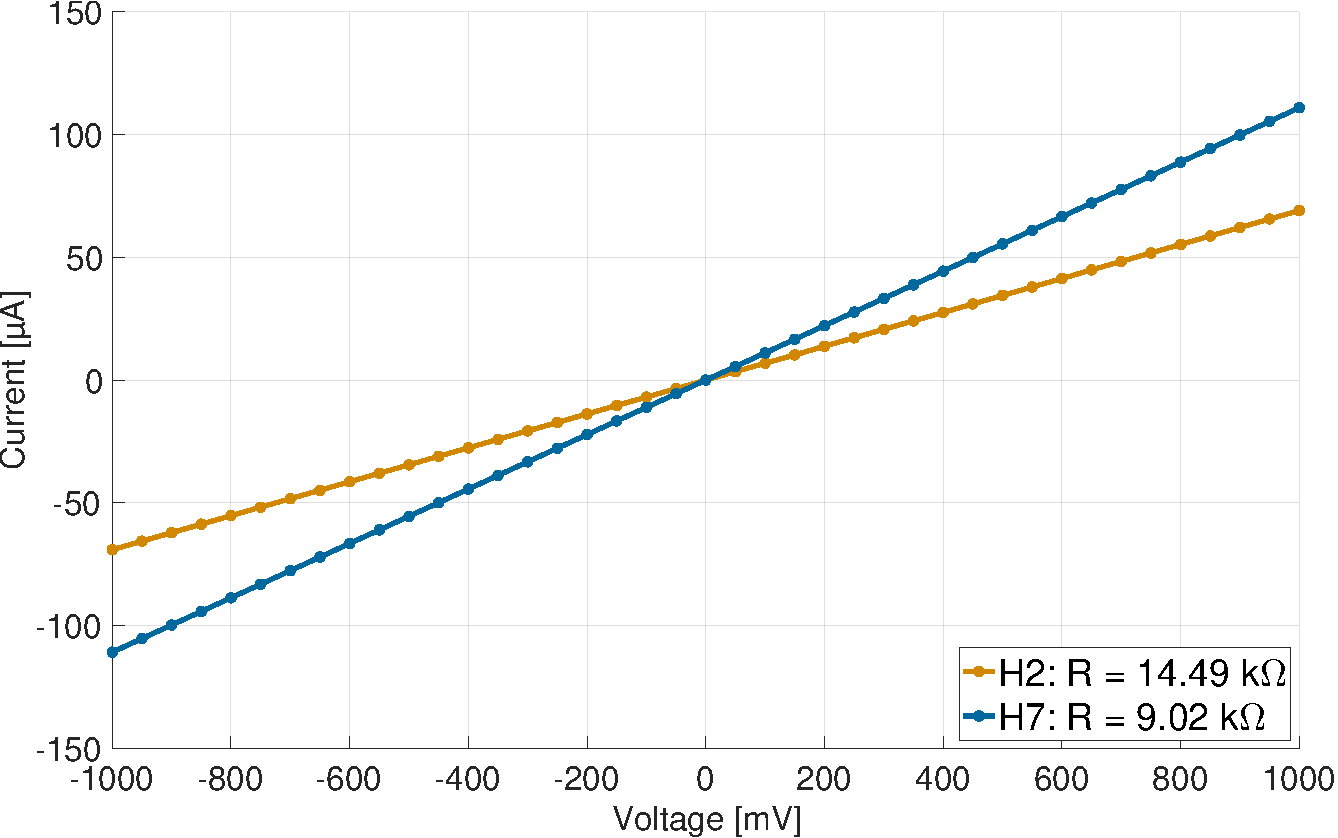
\includegraphics[width=\textwidth]{figures/IV/IV_H2_H7.pdf}
        \caption{IV characteristics of H-Dipole antennas with a NiCr-strip of length $l_{NiCr} = 240$ \si{\micro \meter}.}
        \label{fig:sub2}
    \end{subfigure}
    
    \vspace{1em} % space between rows

    \begin{subfigure}[b]{0.49\textwidth}
        \centering
        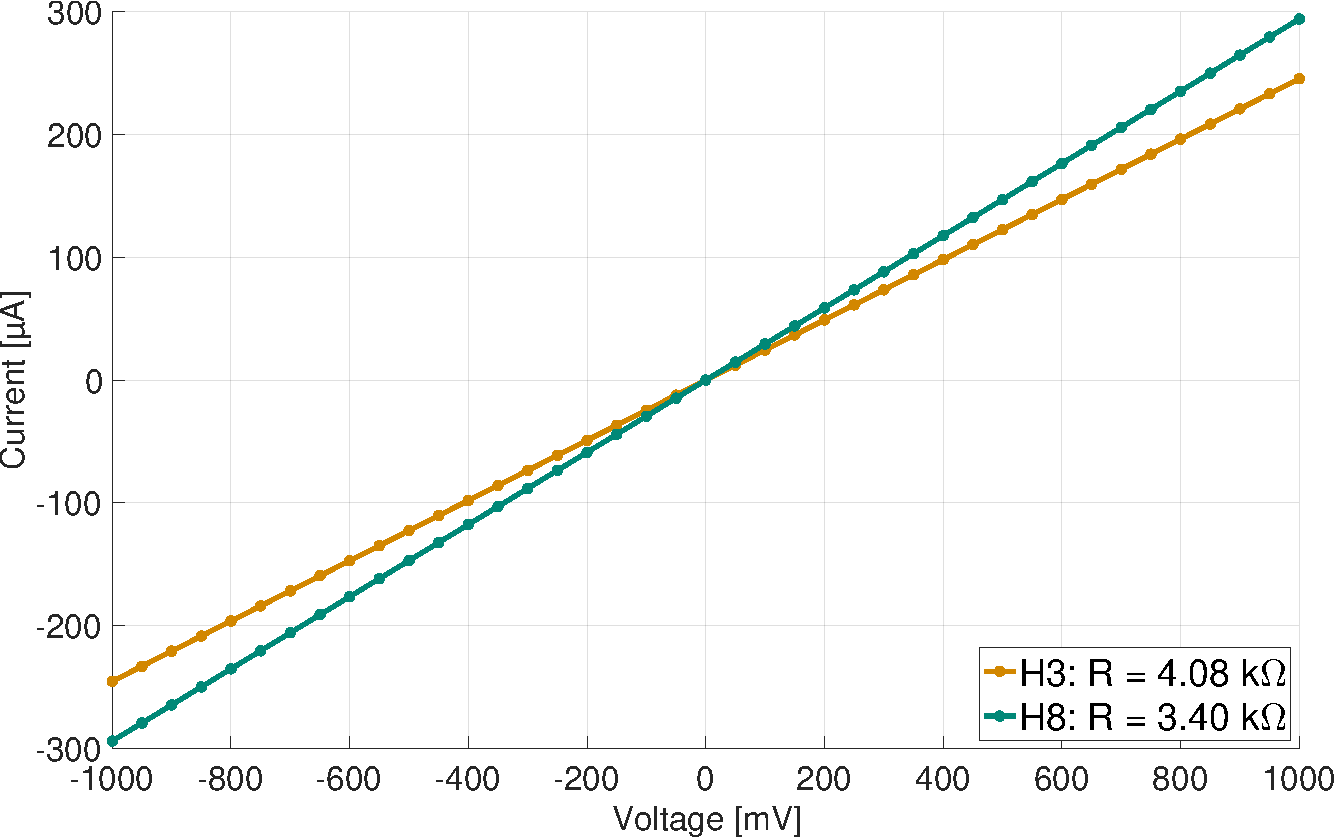
\includegraphics[width=\textwidth]{figures/IV/IV_H3_H8.pdf}
        \caption{IV characteristics of H-Dipole antennas with a NiCr-strip of length $l_{NiCr} = 70$ \si{\micro \meter}.}
        \label{fig:sub3}
    \end{subfigure}
    \hfill
    \begin{subfigure}[b]{0.49\textwidth}
        \centering
        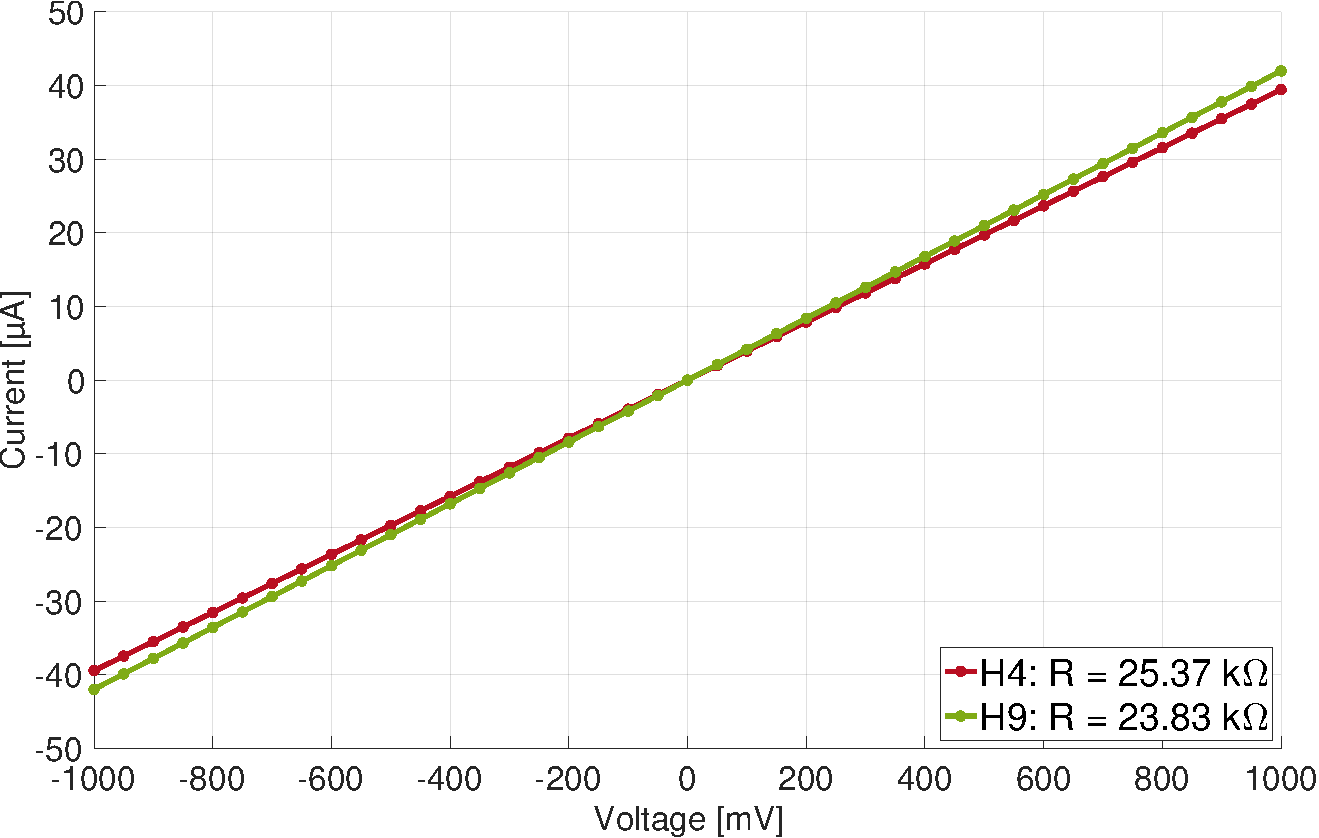
\includegraphics[width=\textwidth]{figures/IV/IV_H4_H9.pdf}
        \caption{IV characteristics of H-Dipole antennas with a NiCr-strip of length $l_{NiCr} = 751$ \si{\micro \meter}.}
        \label{fig:sub4}
    \end{subfigure}
    
    \vspace{1em} % space between rows

    \begin{subfigure}[b]{0.49\textwidth}
        \centering
        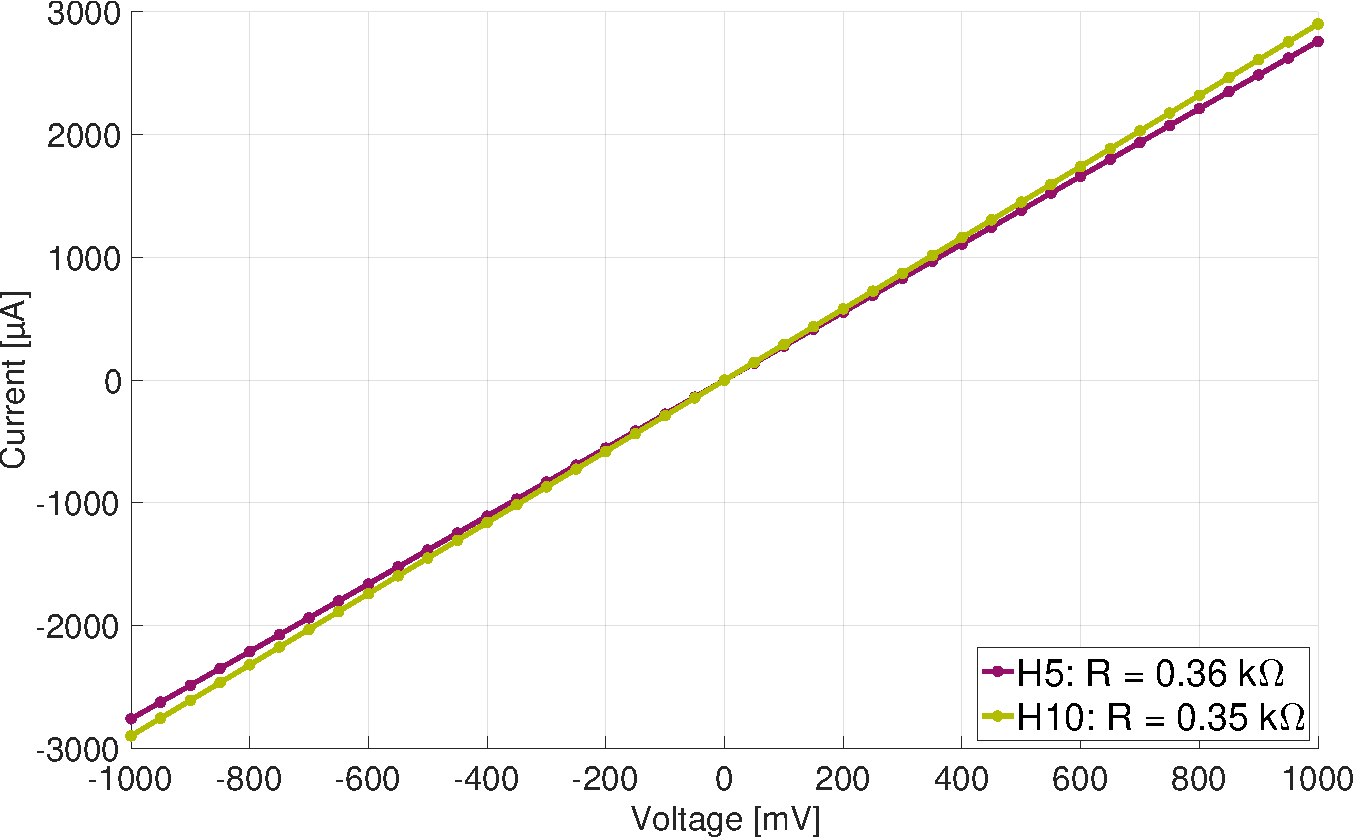
\includegraphics[width=\textwidth]{figures/IV/IV_H5_H10.pdf}
        \caption{IV characteristics of H-Dipole antennas with a NiCr-strip of length without added NiCr.}
        \label{fig:sub5}
    \end{subfigure}

    \caption{Measured IV characteristics of the fabricated H-Dipole antennas.}
    \label{fig:main_IV_dipoles}
\end{figure}
